\subsection{Quickstart}
Die folgenden Schritte zeigen den schnellsten Weg, um \projektname lokal zu starten. Das Setup wird über das Control-/Checkup-Tooling standardisiert (z.\,B. \codeinline{doctor}, \codeinline{install}, \codeinline{run}). 

\begin{codeblock}[title={Quickstart: Clone the repo \& switch to a standard project directory}]
# Standard project directory (works on Linux systems):
mkdir -p ~/Projects
cd ~/Projects

# Clone repository (replace URL)
git clone https://github.com/kleiveist/FMDFlashcard.git
cd FMDFlashcard

# Control-Skript
cd ~/Projects/FMDFlashcard
# optional: health check / doctor
python3 tools/control.py --doctor

# Install & start
cd ~/Projects/FMDFlashcard
python3 tools/control.py --install
\end{codeblock}


\textit{Hinweis:} Das Beispiel oben zeigt die Befehle für ein Linux-System; unter macOS sind \texttt{git clone} und \texttt{cd} identisch. Unter Windows funktionieren die Befehle in \enquote{Git Bash} wie unter Linux; in PowerShell/CMD ebenfalls, nur das Auflisten des Verzeichnisses erfolgt typischerweise mit \texttt{dir} (PowerShell unterstützt auch \texttt{ls}).

Nach dem Ausführen von \texttt{python3 tools/control.py --doctor} wird eine Auflistung der noch fehlenden Pakete und Module angezeigt. Diese werden anschließend automatisch mit folgendem Befehl installiert:

\begin{verbatim}
python3 tools/control.py --install
\end{verbatim}

Nach der Installation wird \texttt{python3 tools/control.py --doctor} erneut ausgeführt. Das Ergebnis ist in Abbildung~\ref{fig:terminal-checkup} dargestellt.

\begin{figure}[H]
    \centering
    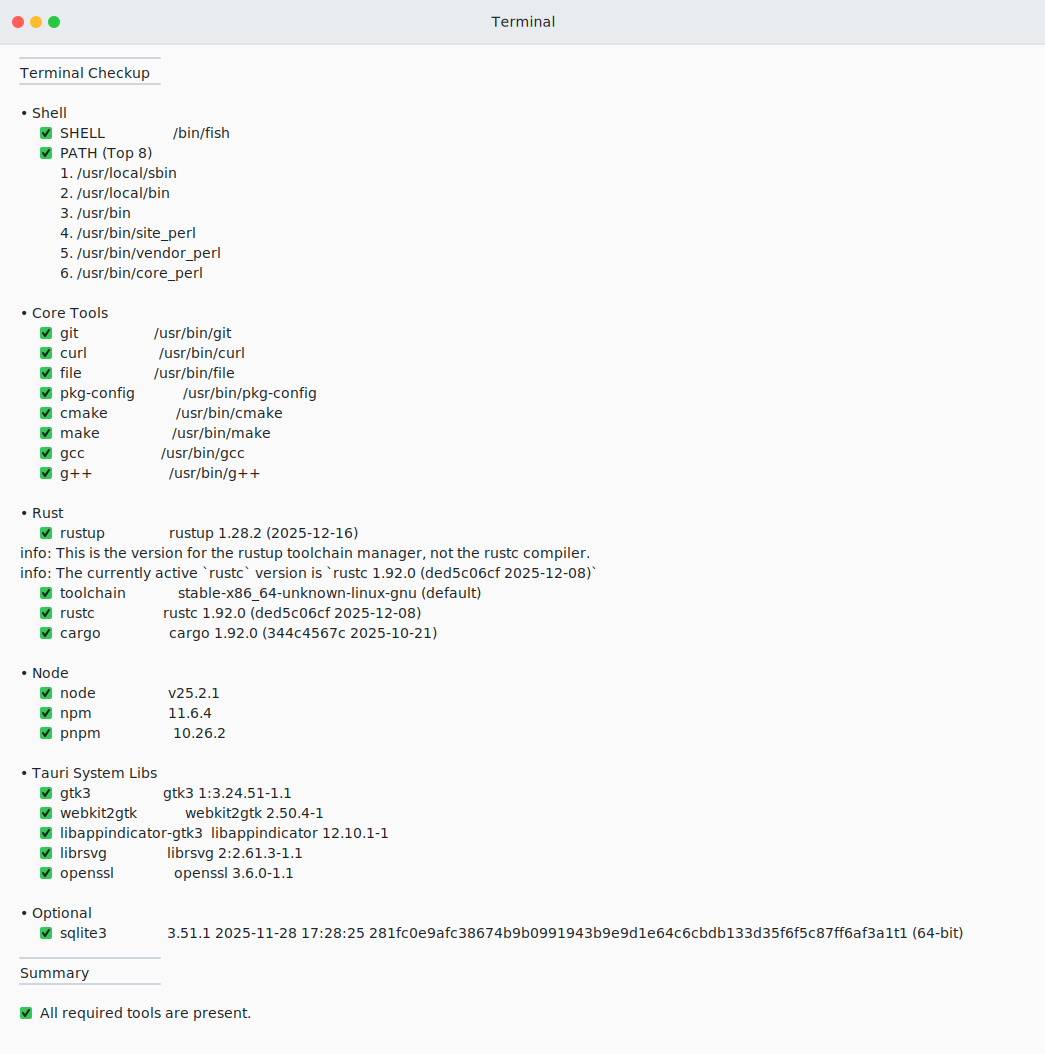
\includegraphics[width=0.9\textwidth]{FMD/image/terminal_checkup_light.png}
    \caption{Terminal Checkup.\cite{Eigendarstellung}}
    \label{fig:terminal-checkup}
\end{figure}



\subsubsection{Terminal Checkup}
In den folgenden Unterabschnitten werden die einzelnen Bereiche der Terminal-Überprüfung erläutert. Ziel ist es, die angezeigten Komponenten kurz einzuordnen und zu begründen, warum diese Prüfungen durchgeführt werden. Dadurch wird sichergestellt, dass alle notwendigen Werkzeuge und Systemabhängigkeiten für Installation, Build und Ausführung der Anwendung vorhanden und korrekt konfiguriert sind.

\subsection{Erläuterung der Checkup-Bereiche}
Die folgenden Punkte erklären die im Terminal-Checkup ausgegebenen Bereiche und deren Zweck.

\begin{itemize}
    \item \textbf{Shell (in den meisten Systemen bereits installiert):}
    Zeigt die verwendete Shell sowie die \texttt{PATH}-Konfiguration. Damit wird geprüft, ob wichtige Programme über die Kommandozeile gefunden werden und die Entwicklungsumgebung korrekt eingerichtet ist.

    \item \textbf{Core Tools (in den meisten Systemen bereits installiert):}
    Enthält grundlegende Entwicklungswerkzeuge (z.\,B. \texttt{git}, Compiler, Build-Tools). Diese werden benötigt, um Quellcode zu beziehen, native Abhängigkeiten zu kompilieren und Build-Prozesse zuverlässig auszuführen.

    \item \textbf{Rust:}
    Prüft die Rust-Toolchain (\texttt{rustup}, \texttt{rustc}, \texttt{cargo}). Dies ist erforderlich, da das Tauri-Backend in Rust gebaut wird und ohne eine passende Toolchain keine Kompilierung und kein Packaging möglich ist.

    \item \textbf{Node:}
    Überprüft Node.js sowie Paketmanager wie \texttt{npm}/\texttt{pnpm}. Diese werden für das Frontend benötigt, um JavaScript-Abhängigkeiten zu installieren und das Web-Bundle für die Tauri-App zu erstellen.

    \item \textbf{Tauri System Libs:}
    Listet systemweite Bibliotheken auf, die unter Linux für WebView und GUI-Funktionalitäten notwendig sind (z.\,B. \texttt{gtk3}, \texttt{webkit2gtk}, \texttt{openssl}). Dadurch wird sichergestellt, dass die Anwendung sowohl gebaut als auch zur Laufzeit korrekt ausgeführt werden kann.
\end{itemize}

\paragraph{Hinweis zu Windows und macOS}
Neben der Linux/Unix-Variante existieren auch Installationsskripte für Windows und macOS, die über die automatische Betriebssystem-Erkennung in \texttt{control.py} referenziert werden (u.\,a. \texttt{installwin.py} und \texttt{installmac.py}). :contentReference[oaicite:0]{index=0}
Diese Skripte sind derzeit jedoch noch nicht in virtuellen Maschinen (VMs) verifiziert bzw. reproduzierbar erprobt worden und gelten deshalb als \textit{ungetestet}. 
